\documentclass[10pt]{article}
\usepackage[english,russian]{babel}
\usepackage{textcomp}
\usepackage[left=2cm, right=2cm, top=1.5cm, bottom=1.5cm]{geometry}
\usepackage{tikz}
\usepackage{multicol}
\usepackage{hyperref}
\usepackage{amsmath}
\usepackage{listings}
\usepackage{colortbl}
\usepackage{graphicx}
\usepackage[shortlabels]{enumitem}
\usepackage{hyperref}
\pagenumbering{gobble}

\lstdefinestyle{CStyle}{
  language=C,
  basicstyle=\linespread{1.1}\ttfamily,
  basewidth=0.5em,
  texcl=true,
  keywordstyle=\color{blue}\bfseries,
  commentstyle=\color{gray},
  stringstyle=\ttfamily\color{orange!50!black},
  showstringspaces=false,
  backgroundcolor=\color{white},
  breaklines=true,
  breakatwhitespace=true,
  xleftmargin=5mm,
  keepspaces = true,
  extendedchars=\true,
  tabsize=4,
  upquote=true,
  emph={size_t, NULL},
  emphstyle={\color{blue}\bfseries},
  literate={~}{{\raisebox{0.5ex}{\texttildelow}}}{1},
}
\lstdefinestyle{boxStyle}{
  style=CStyle,
  framexleftmargin=5mm, 
  frame=shadowbox, 
  rulesepcolor=\color{gray}
}
\lstset{style=CStyle}

\begin{document}
\title{Семинар \#4: Часть 1: Указатели. \vspace{-5ex}}\date{}\maketitle
\section*{Память и адреса}

\textit{Примечание:} Оказывается, что при работе с памятью и адресами удобнее использовать шестнадцатеричную систему счисления, поэтому в этом семинаре мы будем использовать её.\\

Память можно схематично представить как очень большой массив, состоящий из ячеек размером в 1 байт.
Каждая ячейка памяти занумерована. По номеру ячейки можно получить доступ к этой ячейке.
То есть, например, мы можем по номеру ячейки прочитать данные из ячейки или записать туда данные.
Номер ячейки также называется адресом этой ячейки.

Рассмотрим, например, кусок памяти, в которой хранятся какие-то данные:

\begin{center}
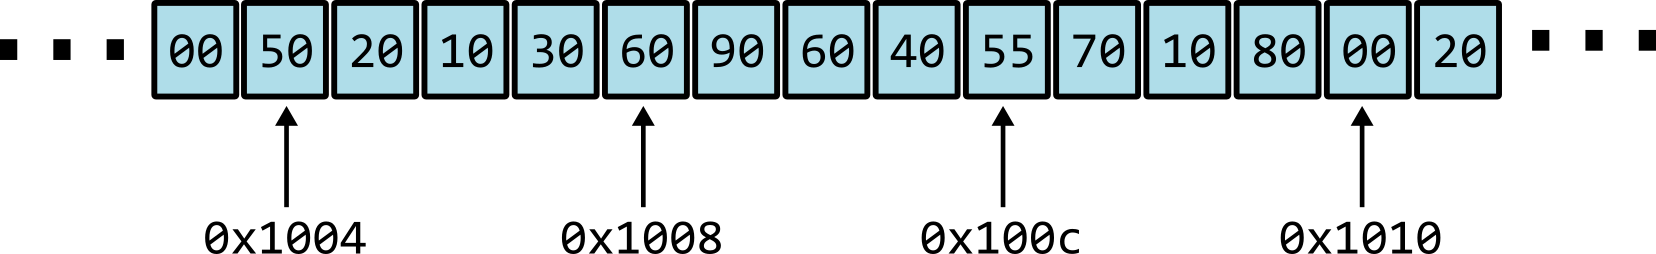
\includegraphics[scale=1]{../images/memory1.png}
\end{center}

 
На участке памяти, изображённом на картинке:

\begin{itemize}
\item Ячейка с адресом 0x1004 хранит однобайтовое число 50
\item Ячейка с адресом 0x1008 хранит однобайтовое число 60
\item Ячейки с адресами от 0x1008 до 0x100c хранят четыре однобайтовые числа  60 90 60 40
\item С другой стороны, в последовательности ячеек от 0x1008 до 0x100c можно хранить одно целое число размером в 4 байта (например \texttt{int}). Или в той же последовательности ячеек от 0x1008 до 0x100c можно хранить число типа \texttt{float}
\end{itemize}

\section*{Адреса переменных}
На большинстве систем переменные типа \texttt{int} занимают 4 байта. Соответственно, если вы создадите 3 переменные типа \texttt{int} вот так:
\begin{lstlisting}
int a = 0x10;   // язык C поддерживает шестнадцатеричную систему счисления
int b = 0x20;   // нужно просто написать 0x перед числом
int c = 0x30;
\end{lstlisting}
то в памяти это может выглядеть примерно вот так:
\begin{center}
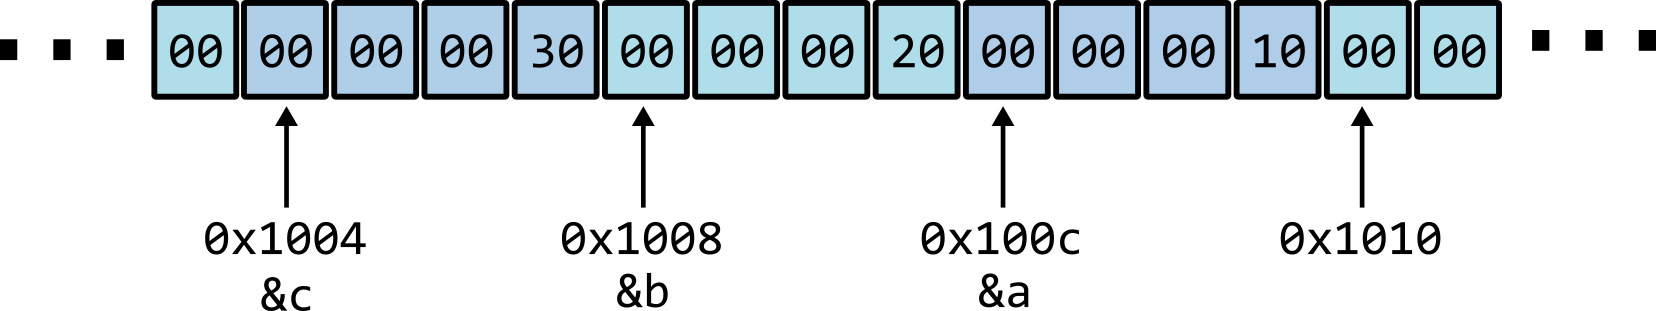
\includegraphics[scale=1]{../images/memory2.png}
\end{center}

Адрес переменной - это адрес первого байта того участка памяти, который занимает данная переменная.
Чтобы получить адрес переменной в языке C нужно написать перед именем переменной символ \texttt{\&}.
Для печати адреса с помощью \texttt{printf} используется спецификатор \texttt{\%p}. 
В этом случае адрес напечатается в шестнадцатеричной системе счисления.
\begin{lstlisting}
int a = 10;
printf("%p\n", &a);
\end{lstlisting}


\section*{Указатели}
Для хранения адресов в языке C введены специальные переменные, которые называются указатели. Тип переменной указателя = тип той переменной, чей адрес он хранит + звёздочка на конце. Например, указатель, который будет хранить адреса переменных типа \texttt{int} должен иметь тип \texttt{int*}. Размер указателя обычно равен размеру машинного слова, то есть на 64-х битных процессорах размер указателя будет равен 8-ми байтам.

Предположим, что определена переменная \texttt{a} и указатель \texttt{p}, хранящий адрес этой переменной:
\begin{lstlisting}
int a = 0x12345678;
int* p = &a;
\end{lstlisting}

В памяти эта ситуация будет выглядеть примерно так:

\begin{center}
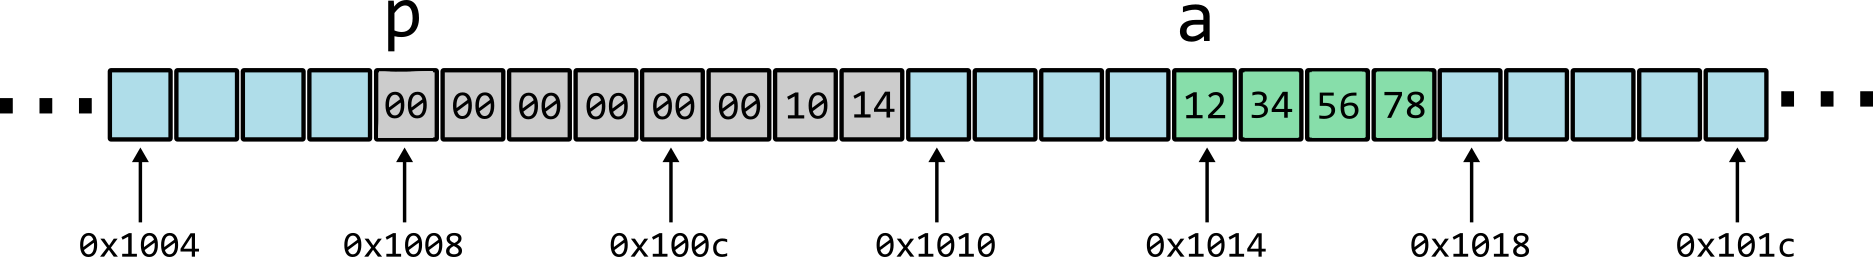
\includegraphics[scale=1]{../images/memory_3_pointer_to_int_b.png}
\end{center}
Примечания:
\begin{itemize}
\item В данном примере для простоты выбраны очень маленькие адреса. В действительности же адрес скорей всего будет очень большим числом.
\item Адреса переменных задаются в момент запуска программы и будут разными при разных запусках.
\item Указатель тоже является переменной и хранится в памяти.
\item На 64-х битных системах указатель обычно занимает 8 байт памяти.
Размер указателя не зависит от размера объекта на который он указывает.
\item Указатель хранит номер одной из ячеек памяти (в данном случае -- первый байт \texttt{a}).
\item Если указатель хранит адрес какого-то объекта, то также говорят, что он \textit{указывает} на этот объект.
\end{itemize}

\subsection*{Операция разыменования}
Разыменование -- это получение самой переменной по указателю на неё. Чтобы разыменовать указатель нужно перед ним поставить звёздочку. То есть, если \texttt{p} это указатель, хранящий адрес \texttt{a}, то \texttt{*p} означает следующее:\\

\textit{Пройди по адресу, хранящемуся в \texttt{p}. Возьми соответствующее количество байт, начиная с этого адреса (в данном случае 4, так как \texttt{p} указывает на \texttt{int}, а размер \texttt{int} равен 4). Воспринимай эти байты как переменную соответствующего типа (в данном случа \texttt{int}).}\\

В примере ниже мы создаём указатель \texttt{p}, хранящий адрес переменной \texttt{a}. Затем, мы используем \texttt{p}, чтобы изменить значение переменной \texttt{a}:
\begin{lstlisting}
#include <stdio.h>
int main() 
{
    int a = 10;
    int* p = &a;
    *p = 20;
    printf("%i\n", a); // Напечатает 20
}
\end{lstlisting}

Не следует путать звёздочку, используемую в операторе разыменования со звёздочкой, используемой при объявлении указателя. 
Это разные звёздочки. Просто так сложилось, что в двух этих случах используется один и тот же символ.
\begin{lstlisting}
int* p = &a;    // Тут звёздочка используется при объявлении указателя. 
                // Она входит в название типа. Тип называется int*

*p = 20;        // Тут звёздочка - это оператор разыменования.
\end{lstlisting}

\newpage
\section*{Примеры}
\begin{enumerate}
\iffalse
\item Пусть есть переменная \texttt{a} типа \texttt{int} и указатель \texttt{p}, хранящий её адрес. Используем переменную \texttt{p}, чтобы увеличить \texttt{a} в 3 раза:
\begin{lstlisting}
#include <stdio.h>
int main() 
{
    int a = 10;
    int* p = &a;
    *p *= 3;
    printf("%i\n", a); // Напечатает 30
}
\end{lstlisting}
\fi

\item Пусть есть переменная \texttt{a} типа \texttt{float} и указатель \texttt{p}, хранящий её адрес. Используем переменную \texttt{p}, чтобы возвести \texttt{a} в квадрат:
\begin{lstlisting}
#include <stdio.h>
int main() 
{
    float a = 1.5;
    float* p = &a;
    *p *= *p;
    printf("%f\n", a); // Напечатает 2.25
}
\end{lstlisting}

\item Пусть есть две переменные \texttt{a} и \texttt{b} и указатель \texttt{p}. Используем \texttt{p}, чтобы прибавить 1 к обоим переменным:
\begin{lstlisting}
#include <stdio.h>
int main() 
{
    int a = 10;
    int b = 20;
    int* p = &a;
    *p += 1;
    p = &b;
    *p += 1;
    printf("%i %i\n", a, b); // Напечатает 11 21
}
\end{lstlisting}

\item Пусть есть переменная \texttt{a} и два указателя \texttt{p} и \texttt{q}, хранящие адрес переменной \texttt{a}. Используем \texttt{p} и \texttt{q}, чтобы увеличить \texttt{a} на 1. 
\begin{lstlisting}
#include <stdio.h>
int main() 
{
    int a = 10;
    int* p = &a;
    int* q = &a;
    *p += 1;
    *q += 1;
    printf("%i\n", a); // Напечатает 12
}
\end{lstlisting}


\item Пусть есть две переменные \texttt{a} и \texttt{b} и указатель \texttt{p}, который хранит адрес \texttt{a}. Пусть также есть указателт \texttt{q}, который хранит адрес \texttt{p}. Используем \texttt{q}, чтобы изменить \texttt{p} так, чтобы он начал хранить адрес переменной \texttt{b}:
\begin{lstlisting}
#include <stdio.h>
int main() 
{
    int a = 10;
    int b = 20;
    int* p = &a;
    printf("%i\n", *p); // Напечатает 10
    
    int** q = &p;
    *q = &b;
    printf("%i\n", *p); // Напечатает 20
}
\end{lstlisting}
\end{enumerate}

\section*{Операции над указателями и арифметика указателей}
С указателями можно производить следующие операции:
\begin{itemize}
\item Разыменование \texttt{*p}
\item Проверка указателей на равенство/неравенство: \texttt{p == q} и \texttt{p != q}
\end{itemize}
Если указатель указывает на один из элементов массива, то к нему также применимы следующие операции:
\begin{itemize}
\item Инкремент \texttt{p++}\\
В этом случае указатель не увеличивается на \texttt{1}, как было можно подумать. Он увеличивается на размер типа, на который он указывает. Таким образом указатель станет указывать на следующий элемент массива.

\item Декремент \texttt{p-{}-}\\
Уменьшается на размер типа, на который он указывает. После этого указатель станет указывать на предыдущий элемент массива.

\item Прибавить или отнять число \texttt{p + k} и \texttt{p - k}\\
В этом случае указатель не увеличивается на \texttt{k}, как было можно подумать. Он увеличивается на \texttt{k * sizeof(*p)}. Если \texttt{p} указывает на \texttt{i}-ый элемент массива, то \texttt{p + k} будет указывать на \texttt{(i + k)}-ый элемент.

\item Вычитание 2-х указателей \texttt{p - q}\\
Вернётся разница между указателями делённая на размер типа указателя.
При этом важно, чтобы оба указателя указывали на элементы одного и того же массива, иначе эта операция приведёт к ошибке.

\item Сравнение 2-х указателей \texttt{p > q} и т. д.\\
Оба указателя должны указывать на элементы одного массива. Указатель больше, если он указывает на элемент с большим индексом.

\item Квадратные скобки \texttt{p[i]}\\
Также как и к массивам, к указателям можно применять квадратные скобочки. Квадратные скобочки эквивалентны прибавлению числа и разыменованию по следующей формуле: \texttt{p[i]} = \texttt{*(p+i)}
\end{itemize}

Используя операторы, приведённые выше важно не выйти за пределы массива. Иначе произойдет ошибка. 

\subsection*{Применение арифметики указателей для доступа к элементам массива}
\begin{lstlisting}
#include <stdio.h>
int main() 
{
    int a[6] = {10, 20, 30, 40, 50, 60};
    
    int* p = &a[0];
    printf("%i\n", *p);       // Напечатает 10
    p++;
    printf("%i\n", *p);       // Напечатает 20
    printf("%i\n", *(p + 2)); // Напечатает 40
    printf("%i\n", p[2]);     // Напечатает 40
}
\end{lstlisting}


\subsection*{Обход массива с помощью указателя}
\begin{lstlisting}
#include <stdio.h>
int main() 
{
    int a[6] = {10, 20, 30, 40, 50, 60};
    for (int* p = &a[0]; p <= &a[5]; ++p) 
        printf("%i\n", *p);
}
\end{lstlisting}



\newpage

\section*{Схематическое изображение указателей в памяти}
Так как постоянно рисовать переменные в памяти слишком громоздко и затруднительно, будем изображать их схематически. Указатели будем изображать серым прямоугольником, а другие переменные -- прямоугольниками другого цвета. Стрелочкой будем указывать на переменную, адрес которой хранит указатель. Размеры прямоугольников не соответствуют размерам переменных.

Например, переменные из следующей программы:

\begin{lstlisting}
#include <stdio.h>
int main() 
{
    int a = 123;
    int* p = &a;
    printf("%i\n", *p); // Напечатает 123
}
\end{lstlisting}

будем изображать вот так:

\begin{center}
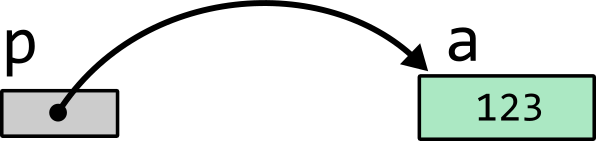
\includegraphics[scale=1]{../images/memory_3_pointer_to_int_b_scheme.png}
\end{center}
\subsubsection*{Задачи:}
Напишите код, который будет соответствовать следующим рисункам. В каждой задаче разыменуйте указатели и напечатайте то, на что они указывают.
\begin{itemize}
\item Указатель на переменную типа \texttt{char}.
\begin{center}
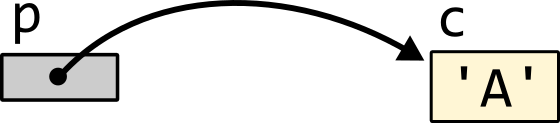
\includegraphics[scale=1]{../images/pointer_tasks/pointer_task_char.png}
\end{center}

\item Два указателя, которые указывают на одну переменную типа \texttt{int}
\begin{center}
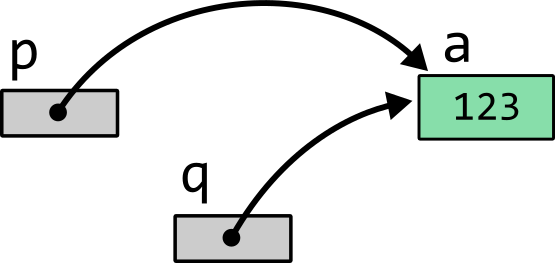
\includegraphics[scale=1]{../images/pointer_tasks/pointer_tasks_two_int.png}
\end{center}

\item Указатель типа \texttt{int*}, указывает на первый элемент массива \texttt{int}-ов под названием \texttt{array}
\begin{center}
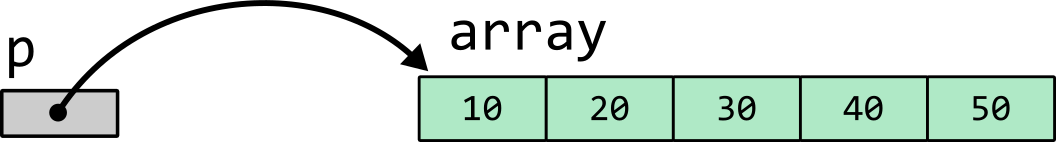
\includegraphics[scale=1]{../images/pointer_tasks/pointer_task_array.png}
\end{center}

\item Указатель типа \texttt{int*}, указывает на четвёртый элемент массива \texttt{int}-ов под названием \texttt{array}
\begin{center}
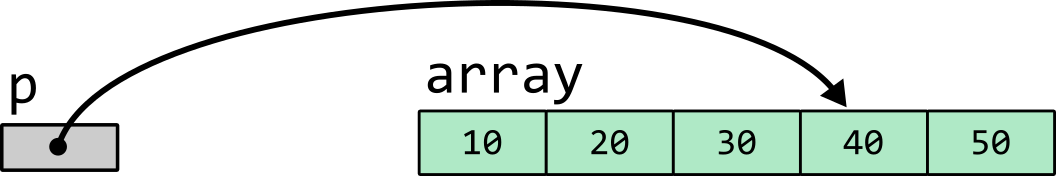
\includegraphics[scale=1]{../images/pointer_tasks/pointer_task_array_4.png}
\end{center}


\item Указатель типа \texttt{int**}, указывает на указатель \texttt{int*}, который указывает на переменную типа \texttt{int}.
\begin{center}
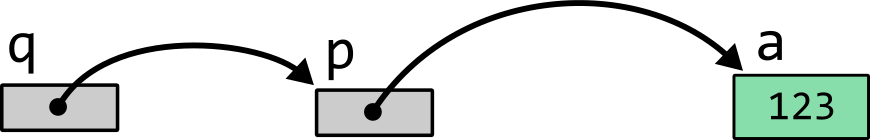
\includegraphics[scale=1]{../images/pointer_tasks/pointer_tasks_pointer_to_pointer.png}
\end{center}
\end{itemize}



\newpage



\newpage
\section*{Передача в функцию по указателю}
Указатели, как и другие переменные, можно передавать в функции.
Например, функция \texttt{print\_address} из примера ниже принимает на вход указатель на \texttt{int} и печатает значение этого указателя на экран:
\begin{lstlisting}
#include <stdio.h>

void print_address(int* p)
{
    printf("%p\n", p);
}

int main()
{
    int a = 10;
    print_address(&a);
}
\end{lstlisting}

Как известно, что любое выражение, которое мы передаём в функцию копируется (за исключением массивов). Указатели, как и обычные переменные, копируются в функции. Но что означает копия указателя? Если один указатель хранит адрес некоторой переменной, то и его копия будет хранить адрес той же самой переменной. Поэтому, передавая в функцию не саму переменную, а указатель на эту переменную, мы можем менять саму переменную внутри, используя указатель.

\begin{multicols}{2}
\noindent
\begin{lstlisting}
#include <stdio.h>

void inc(int* p)
{
    // p хранит адрес переменной a
    *p += 1; 
}

int main()
{
    int a = 10;
    int* p = &a;
    inc(&a);
    printf("%i\n", a); // Напечатает 11
}
\end{lstlisting}

\begin{center}
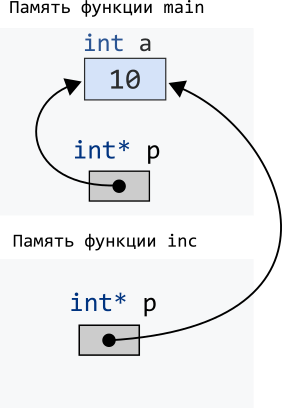
\includegraphics[scale=0.62]{../images/intpassbypointer.png}
\end{center}
\end{multicols}

\section*{Примеры}

\begin{enumerate}
\iffalse
\item Функция, которая адреса переменной типа \texttt{float} и умножает значение этой переменной на 2:
\begin{lstlisting}
#include <stdio.h>

void mult2(float* p)
{
    *p *= 2;
}

int main()
{
    float a = 1.23;
    mult2(&a);
    printf("%lf\n", a); // Напечатает 2.46
}
\end{lstlisting}
\fi

\item Функция, которая принимает адреса двух переменных и возвращает их сумму:
\begin{lstlisting}
#include <stdio.h>

int add(int* pa, int* pb)
{
    return *pa + *pb;
}

int main()
{
    int a = 10;
    int b = 20;
    printf("%i\n", add(&a, &b)); // Напечатает 30
}
\end{lstlisting}


\item Функция, которая принимает адреса двух переменных и меняет их значения местами:
\begin{lstlisting}
#include <stdio.h>

void swap(int* pa, int* pb)
{
    int temp = *pa;
    *pa = *pb;
    *pb = temp;
}

int main()
{
    int a = 10;
    int b = 20;

    printf("%i %i\n", a, b);  // Напечатает 10 20
    swap(&a, &b);
    printf("%i %i\n", a, b);  // Напечатает 20 10
}
\end{lstlisting}

\item Используя указатели в качестве параметров функции, можно добиться того, что функция будет "как бы возвращать" \space более одного значения. Например, в примере ниже написана функция, которая принимает два числа и "возвращает" \space 2 значения: минимум и максимум из этих двух чисел.

\begin{lstlisting}
#include <stdio.h>

void calculate_maxmin(int a, int b, int* pmin, int* pmax)
{
    if (a > b)
    {
        *pmax = a;
        *pmin = b;
    }
    else
    {
        *pmax = b;
        *pmin = a;
    }
}

int main()
{
    int max, min;
    calculate_maxmin(10, 20, &min, &max);
    printf("min = %i, max = %i\n", min, max);

    calculate_maxmin(90, 70, &min, &max);
    printf("min = %i, max = %i\n", min, max);
}
\end{lstlisting}
\end{enumerate}



\newpage
\section*{Указатели и массивы. Array to pointer decay.}
При передаче в функцию массива, туда на самом деле передаётся указатель на первый элемент этого массива.
\begin{lstlisting}
#include <stdio.h>
void func(int a[5]) 
{
    printf("%zu\n", sizeof(a)); // Напечатает 8, так как a тут это указатель
}
int main() 
{
    int x[5] = {10, 20, 30, 40, 50};
    printf("%zu\n", sizeof(x));   // Напечатает 20, так как x это массив из пяти int - ов
    func(x);
}
\end{lstlisting}

Получается, что когда мы передаём в функцию массив, туда на самом деле передаётся указатель на первый элемент. Можно сказать, что внутри функции массив как бы превращается в указатель. Такое необычное явление в языке называется \textit{array to pointer decay} (\textit{разложение массива в указатель}).
При этом, пользоваться указателем \texttt{a} в функции \texttt{func} можно почти также как и массивом, так как к указателям тоже применимы квадратные скобочки.
Чтобы не путать в дальнейшем тип параметра, будем всегда для функций, принимающих массив, явно прописывать тип указателя. Например, функцию \texttt{func} из примера выше будем писать так:
\begin{lstlisting}
void func(int* a) 
{
    printf("%zu\n", sizeof(a));
}
\end{lstlisting}

Большой недостаток автоматической передачи массива через указатель заключается в том, что мы никак не можем узнать размер передаваемого массива:

\begin{lstlisting}
void func(int* a) 
{
    // Не можем узнать размер массива
}
int main() 
{
    int x[5] = {10, 20, 30, 40, 50};
    printf("%zu\n", sizeof(x) / sizeof(x[0])); // Можем узнать размер массива
    func(x);
}
\end{lstlisting}

Единственный вариант -- это передавать размер массива через параметр функции:
\begin{lstlisting}
void func(int* a, size_t n) 
{
    printf("%zu\n", n);
}
\end{lstlisting}

\subsection*{Передача строк в функцию}
Строки -- это по сути массивы элементов типа \texttt{char}. Но конец строки задаётся специальным нулевым символом, поэтому нам не нужно передавать размер строки в функцию отдельным параметром. Мы можем просто узнать размер, например используя функцию \texttt{strlen}.
\begin{lstlisting}
void func(char* a) 
{
    printf("%zu\n", strlen(a));
}
\end{lstlisting}


\newpage
\section*{Возврат указателя из функции. Висячие указатели}
Указатели можно также возвращать из функций, но делать нужно с осторожностью, так как в этом случае легко написать некорректную программу. . Рассмотрим, например, следующий пример, в котором из функции \texttt{func} возвращается адрес локальной переменной \texttt{a}. 
\begin{lstlisting}
#include <stdio.h>
int* func() 
{
    int a = 10;
    int* p = &a;
    return p;
}
int main() 
{
    int* q = func();
    printf("%i\n", *q); // Ощибка (UB)
}
\end{lstlisting}
Эта программа некорректна. Дело в том, что из функции \texttt{func} возвращается адрес локального объекта \texttt{a}, но все локальные объекты уничтожаются во время выхода из функции. То есть после того как функция \texttt{func} отработала, её локальные переменные (\texttt{a} и \texttt{p}) уничтожатся. В результате в указателе \texttt{q} будет хранится адрес уже несуществующей переменной \texttt{a}. Такой указатель называют висячим.
\begin{center}
\textit{Висячий указатель (англ. dangling pointer) -- это указатель, указывающий на несуществующий объект.}
\end{center}
Разыменование такого указателя приведёт к тому, что вся ваш программа станет некорректной.
Возникнет особая ситуация, называемая неопределённым поведением (англ. undefined behavior или UB). 
Опасность этой ситуации в том, что код может скомпилироваться без предупреждений и ошибок, но программа может работать не так как надо. В результате такую ошибку будет очень сложно обнаружить и исправить.

Тем не менее, есть ситуации, когда возвращать указатель из функции можно. Главное, чтобы объект, адрес которого мы возвращаем, продолжал существовать после завершения функции.

\begin{multicols}{2}
\noindent
Возвращаем адрес глобальной переменной:
\begin{lstlisting}
#include <stdio.h>

int x = 10;

int* func() 
{
    return &x;
}

int main() 
{
    int* q = func();
    printf("%i\n", *q); // 10
}
\end{lstlisting}
\columnbreak
Возвращает адрес переменной из памяти \texttt{main}:
\begin{lstlisting}
#include <stdio.h>

int* func(int* p) 
{
    *p += 1;
    return p;
}

int main() 
{
    int x = 10;
    int* q = func(&x);
    printf("%i\n", *q); // 11
}
\end{lstlisting}


\end{multicols}

\newpage
\section*{Константные указатели}
! Терминология в этом вопросе может отличаться в разных курсах/книгах.\\

В случае указателя мы можем потребовать сделать неизменяемым две разные величины: сам указатель и объект, на который он указывает. 
Указатель, который не может меняться сам, но при этом, используя этот указатель, можно поменять то, на что он указывает, будем называть \textit{постоянным указателем}. Такой указатель можно объявить следующим образом:
\begin{lstlisting}
int* const p = &a;
\end{lstlisting}

Указатель, который можно менять, но, используя его, нельзя изменить то, на что он указывает, будем называть \textit{константным указателем}. Такой указатель можно объявить следующим образом:
\begin{lstlisting}
const int* p = &a;
\end{lstlisting}

\begin{multicols}{2}
Постоянный указатель
\begin{lstlisting}
int a = 10;
int b = 20;
int* const p = &a;
p = &b;   // Error
*p += 1;  // OK
\end{lstlisting}

Константный указатель
\begin{lstlisting}
int a = 10;
int b = 20;
const int* p = &a;
p = &b;   // OK
*p += 1;  // Error
\end{lstlisting}
\end{multicols}

Как запомнить какой указатель что делает неизменяемым:
\begin{lstlisting}
int* <@\textcolor{red}{const p}@> = &a;  // p нельзя изменить
<@\textcolor{red}{const int}*@> p = &a;  // int нельзя изменить
\end{lstlisting}


\section*{Указатели разных типов}
Как вы могли заметить, тип указателя зависит от типа элемента на который он указывает. Но все указатели, независимо от типа, по сути хранят одно и то же (адрес первого байта объекта). 

Например, если у нас есть указатель типа \texttt{int*}, который указывает на объект типа \texttt{int} (размер \texttt{int} равен 4 байта), то в памяти это может быть выглядеть примерно так:
\begin{lstlisting}
int a = 0x12345678;
int* p = &a;
\end{lstlisting}

\begin{center}
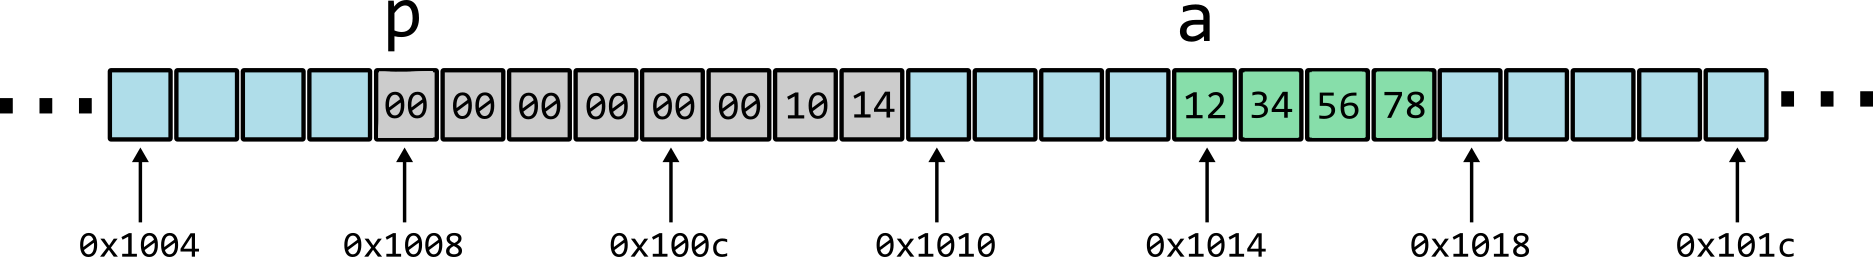
\includegraphics[scale=1]{../images/memory_3_pointer_to_int_b.png}
\end{center}

Если же у нас есть указатель типа \texttt{char*}, указывающий на объект типа \texttt{char} (размер \texttt{char} равен 1 байт), то в памяти это будет выглядеть примерно так:
\begin{lstlisting}
char a = 'A'; // Код символа 'A' равени 0x41 
char* p = &a;
\end{lstlisting}

\begin{center}
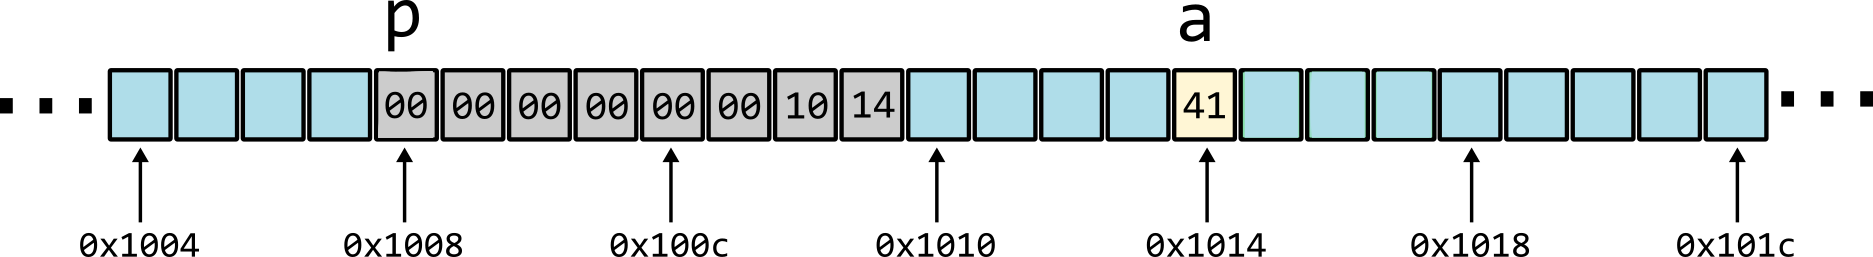
\includegraphics[scale=1]{../images/memory_3_pointer_to_char_b.png}
\end{center}

\newpage
В чём отличие между указателем типа \texttt{int*} и указателем типа \texttt{char*}? Разница проявляется в двух случаях:
\begin{enumerate}
\item При разыменовывание\\
При разыменовывании указатель \texttt{int*} берёт 4 байта, начиная с адреса, который он хранит, и воспринимает эти байты как переменную типа \texttt{int}, Указатель \texttt{char*} берёт 1 байт по адресу, который он хранит, и воспринимает его как переменную типа \texttt{char}.

\item При использовании арифметики указателей\\
Если прибавить к указателю типа \texttt{int*} число \texttt{1}, то его значение увеличится на \texttt{1 * sizeof(int)}, то есть на 4 байта. Указатель из примера выше после такого будет иметь значение \texttt{0x1018}. Если же прибавить \texttt{1} к указателю типа \texttt{char*} то он увеличится на \texttt{1 * sizeof(char)}, то есть на 1 байт. Указатель из примера выше после такого будет иметь значение \texttt{0x1015}.
\end{enumerate}

\subsection*{Приведение типов указателей}
Указатели можно преобразовывать из одного типа в другой. Это похоже на преобразование типов обычных переменных.
\begin{lstlisting}
int a = 4.1;         // Неявное преобразование из double в int
int b = (int)4.1;    // Явное преобразование из double в int

char* p = &a;        // Неявное преобразование из int* в char*  ( не работает в C++ )
char* p = (char*)&a; // Явное преобразование  из int* в char*
\end{lstlisting}
Надо отметить, что язык \texttt{C++} строже относится к соблюдению типов, чем язык \texttt{C}, и не позволит вам неявно преобразовать указатель одного типа в указатель другого типа.


\subsection*{Указатель \texttt{void*}}
Особый указатель \texttt{void*} не ассоциирован ни с каким типом:
\begin{lstlisting}
int a = 10;
void* p = &a;  // Просто хранит адрес переменной a
\end{lstlisting}
Такой указазатель нельзя разыменовать и к нему нельзя применять арифметику указателей.
Чтобы использовать объект, на который указывает \texttt{void*}, нужно сначала привести указатель к необходимому типу:
\begin{lstlisting}
*(int*)p = 20;     // Преобразовали void* в int* и затем разыменовали
printf("%i\n", a);  // Напечатает 20
\end{lstlisting}



\newpage
\section*{Замечания по поводу синтаксиса объявления указателей}
\subsection*{Объявление нескольких указателей в одной строке}
Допустим мы захотели создать несколько указателей одного типа, например \texttt{int*}. Это можно сделать так:
\begin{lstlisting}
int* p;
int* q;
\end{lstlisting}
Но что если мы хотим сократить эту запись и создать 2 указателя в одной строке, вот так:
\begin{lstlisting}
int* p, q;
\end{lstlisting}

Кажется, что и \texttt{p} и \texttt{q} будут иметь тип \texttt{int*}, но это не так.
На самом деле, в этом случае \texttt{p} будет иметь тип \texttt{int*}, а \texttt{q} будет иметь тип \texttt{int}.
Чтобы создать два указателя в одной строке, нужно написать так:
\begin{lstlisting}
int* p, * q
\end{lstlisting}
Или так:
\begin{lstlisting}
int *p, *q;
\end{lstlisting}
То есть нужно ставить звёздочку перед каждым именем переменной.\\

Такой странный синтаксис при объявлении указателей существует в языке из-за некоторых
решений создателей языка C при его создании. Чтобы не допускать ошибок при объявлении указателей нужно придерживаться всего одного простого правила:

\begin{center}
\textit{Не объявляйте несколько указателей в одной строке}
\end{center}

Если вам нужно создать несколько указателей, то потратьте по одной строке на объявление указателя.
Это правило является одним из правил хорошего стиля и относится не только к указателям, но и к переменным других типов: структурам, массивам и даже простым числам. Также это правило хорошего тона верно для большинства других языков программирования (в том числе C++).

Единственное исключение из этого правила - это числовые переменные, которые сильно связаны друг с другом:
\begin{lstlisting}
float x, y, z;          // Допустимо
float distance, speed;  // Недопустимо, так как distance и speed не сильно связаны
\end{lstlisting}


\subsection*{Разные варианты синтаксиса объявления указателей}
Если вы посмотрите код, написанный другими программистами, то увидите, что разные программисты используют разный синтаксис при объявлении указателя. Грубо говоря, разные программисты ставят звёздочку в разных местах при объявлении указателей.\\
Допустим мы хотим создать указатель типа \texttt{int*}. Есть 3 распространённых варианта:
\begin{multicols}{3}
\noindent
\begin{lstlisting}
int* p;
\end{lstlisting}

\begin{lstlisting}
int *p;
\end{lstlisting}

\begin{lstlisting}
int * p;
\end{lstlisting}

\end{multicols}

Все эти 3 способа делают одно и то же, а именно создают переменную типа \texttt{int*} по имени \texttt{p}. Преимущества и недостатки каждого из этих методов:
\begin{enumerate}
\item \texttt{int* p}
\begin{itemize}
\item Преимущества:
\begin{itemize}
\item Пишем именно то, что происходит. Мы тут пишем, что создаём переменную типа  \texttt{int*}  по имени \texttt{p}, это именно то, что происходит.
\item Самый понятный способ, значит, если вы будете использовать этот способ, то и ваш код будет более понятным.
\end{itemize}

\item Недостатки:
\begin{itemize}
\item Можно ошибиться при объявлении нескольких указателей в одной строке.
\item Не очень удобно объявлять указатели на функции.
\end{itemize}
\end{itemize}


\item \texttt{int *p}
\begin{itemize}
\item Преимущества:
\begin{itemize}
\item Удобнее объявлять несколько указателей в одной строке.
\item Удобнее объявлять указатели на функции.
\end{itemize}

\item Недостатки:
\begin{itemize}
\item Пишем не то, что происходит. Кажется что мы тут создаём переменную типа \texttt{int}, по имени \texttt{*p}, но это не то, что происходит.
\item Ваш код будет менее понятным.
\end{itemize}
\end{itemize}


\item \texttt{int * p}
\begin{itemize}
\item Преимущества:
\begin{itemize}
\item Нет.
\end{itemize}

\item Недостатки:
\begin{itemize}
\item Совмещает в себе недостатки двух предыдущих способов.
\item Иногда можно спутать с умножением.
\end{itemize}
\end{itemize}

\end{enumerate}

\subsection*{Рекомендации хорошего стиля от создателей языков}
\begin{itemize}
\item В языке C нет рекомендаций от создателей языка, какой способ использовать.
Большинство программистов используют или 1-й или 2-й способ.
\item В языке C++ есть рекомендация от создателей языка (называется C++ Core Guidelines).
Рекомендуется использовать 1-й способ.
\end{itemize}

В этом курсе будет использоваться 1-й способ, а также правило хорошего стиля, которое запрещает объявлять несколько указателей в одной строке.
\end{document}